% MAREA manuscript — working draft.
% Build: bash build.sh   (MiKTeX; elsarticle, numbered citations, elsarticle-num)
% Every number here traces to a notebook, a script or results/*.json; every
% literature claim to literature_quotes.md (verbatim passages with pages).
\documentclass[final,5p,times,number]{elsarticle}

\usepackage{amsmath,amssymb}
\usepackage{graphicx}
\usepackage{booktabs}
\usepackage[hidelinks]{hyperref}
\graphicspath{{figures/}{../figures/}{../figures/tide_comparison/}{../figures/onepixel/}}

% target journal is a placeholder until decided
\journal{Remote Sensing of Environment}

\begin{document}

\begin{frontmatter}

\title{Timing the tide from space: intertidal topography from Sentinel-2
  with the estuarine tide measured from the imagery itself}
% alternative titles kept in draft.md

% TODO: confirm names, order and affiliations
\author[a]{Jorge Alias \'Alvarez\corref{cor1}}
\author[b]{[Supervisor 1]}
\author[c]{[Supervisor 2]}
\cortext[cor1]{Corresponding author}
\affiliation[a]{organization={[Affiliation 1]}, city={Oviedo}, country={Spain}}
\affiliation[b]{organization={[Affiliation 2]}, country={Spain}}
\affiliation[c]{organization={[Affiliation 3]}, country={Spain}}

\begin{abstract}
Tidal flats are among the most extensive and most threatened coastal
ecosystems, and satellite archives now allow their topography to be mapped
by reading, for every pixel, the water level at which it floods. Every
published implementation assigns each scene a single water level, taken
from an ocean tide model or a tide gauge at one point. Inside estuaries
that level is wrong: the tide arrives later and deformed the farther it
travels up the channel, so the error grows inland and is systematic. We
present MAREA, a method that measures this interior lag from the imagery
itself. Each intertidal pixel is treated as a binary tide gauge, and for
each band of along-channel distance the lag that best explains its
ten-year wet/dry record is found by maximising a profiled Bernoulli
likelihood anchored at the mouth. A binary archive can measure the phase
of the interior tide but not its amplitude or datum, and a lag is applied
only where it exceeds what a null world without interior tide would
produce. Tested on four European estuaries against held-out tide gauges,
MAREA recovered lags of 71 and 128~min on the Ems-Dollard and the Wadden
Sea (gauges: 65 and 95), applied none where none exists, and reduced the
water-level error inside those estuaries by more than 40\,\%. Against the
official Dutch bathymetry the elevation error fell by 25--33\,\%, and the
relief at the head of the Ems-Dollard, absent from the uncorrected map, was
recovered. Against an RTK-GNSS survey in the R\'ia de Villaviciosa (Spain)
the estimator reached 0.16~m, half the error of the published logistic
alternative. The method needs no instrument inside the estuary; code,
notebooks and negative results are released.
\end{abstract}

\begin{keyword}
intertidal topography \sep tidal flats \sep Sentinel-2 \sep tidal
propagation \sep estuaries \sep waterline method \sep tide models \sep
profile likelihood \sep digital elevation model
\end{keyword}

\end{frontmatter}

% Highlights (Elsevier asks for them as a separate file at submission; the
% text is kept in draft.md, not in the manuscript body).

\section{Introduction}

Tidal flats are one of the most extensive coastal ecosystems and, until
recently, one of the least mapped: the first global inventory found at
least 127\,921~km$^2$ of them and a loss of 16\,\% between 1984 and 2016
wherever the record allows a trend \citep{murray2019}. They are highly
productive, host migratory shorebirds and buffer the coast against storms
\citep{sagar2017}, and almost everything about them depends on elevation:
how often each point is flooded, which habitat it can hold, how sediment
moves, how far a surge reaches. Yet detailed coastal topography remains
coarse, outdated or absent over large parts of the world
\citep{almar2021}, because surveying a mudflat is slow, expensive and
often dangerous, with soft substrate and short exposure windows
\citep{bell2016,sagar2017}. Global surface-water products ignore the
tidal stage of each image \citep{pekel2016,fitton2021}, a sun-synchronous
orbit samples the tide unevenly \citep{eleveld2014}, and even habitat
mapping from Sentinel-2 is limited by the scarcity of clear, low-tide
scenes: four usable images a year at Santander Bay, on the coast studied
here \citep{davies2024}.

The satellite archive offers a way round the survey: the tide itself scans
the relief. A pixel is wet when the water stands above it and dry when it
stands below, so a dated series of images is a series of yes/no questions
about the elevation of every pixel. Two lineages of methods exploit this.
The waterline approach, introduced with airborne radar and then satellite
imagery \citep{mason1995,ryu2008}, extracts the land--water contour of each
scene, tags it with the water level at acquisition and interpolates a
surface between contours \citep{sagar2017,bishoptaylor2019ecss,fitton2021}, with
sub-pixel refinements of the contour itself
\citep{bishoptaylor2019waterline,vos2019}; it produced the first
continental intertidal elevation models of Australia
\citep{sagar2017,bishoptaylor2019ecss} and a product for the United
Kingdom and Ireland \citep{fitton2021}. The per-pixel approach instead
fits, to each pixel's radiometry against water level, a logistic curve
whose midpoint is the elevation: first with X-band SAR backscatter
\citep{catalao2017}, then with Sentinel-2 near-infrared reflectance
\citep{bue2020,granadeiro2021}, and most recently with a logistic
regression on the binary water/land class \citep{chen2025}; a temporal
variant cross-correlates radar intensity series with the wet/dry sequence
each candidate elevation would produce \citep{bell2016}. All of these
curves are dose--response ogives in the sense of the quantal-response
curves of Gaddum~\cite{gaddum1933} and Bliss~\cite{bliss1934}, later
formalised as probit and logit analysis \citep{finney1947,berkson1944}:
the flooded fraction of a pixel is the cumulative distribution of its
internal relief, and the 50\,\% point is its elevation, because at medium resolution
a shoreline pixel is a mixture whose index value tracks the proportion of
water in it \citep{rover2010,feyisa2014,bishoptaylor2019waterline}.
Figure~\ref{fig:flats} shows what is being mapped: ground that a person
can walk across at low water and that lies under metres of water a few
hours later.

\begin{figure}[t]
\centering
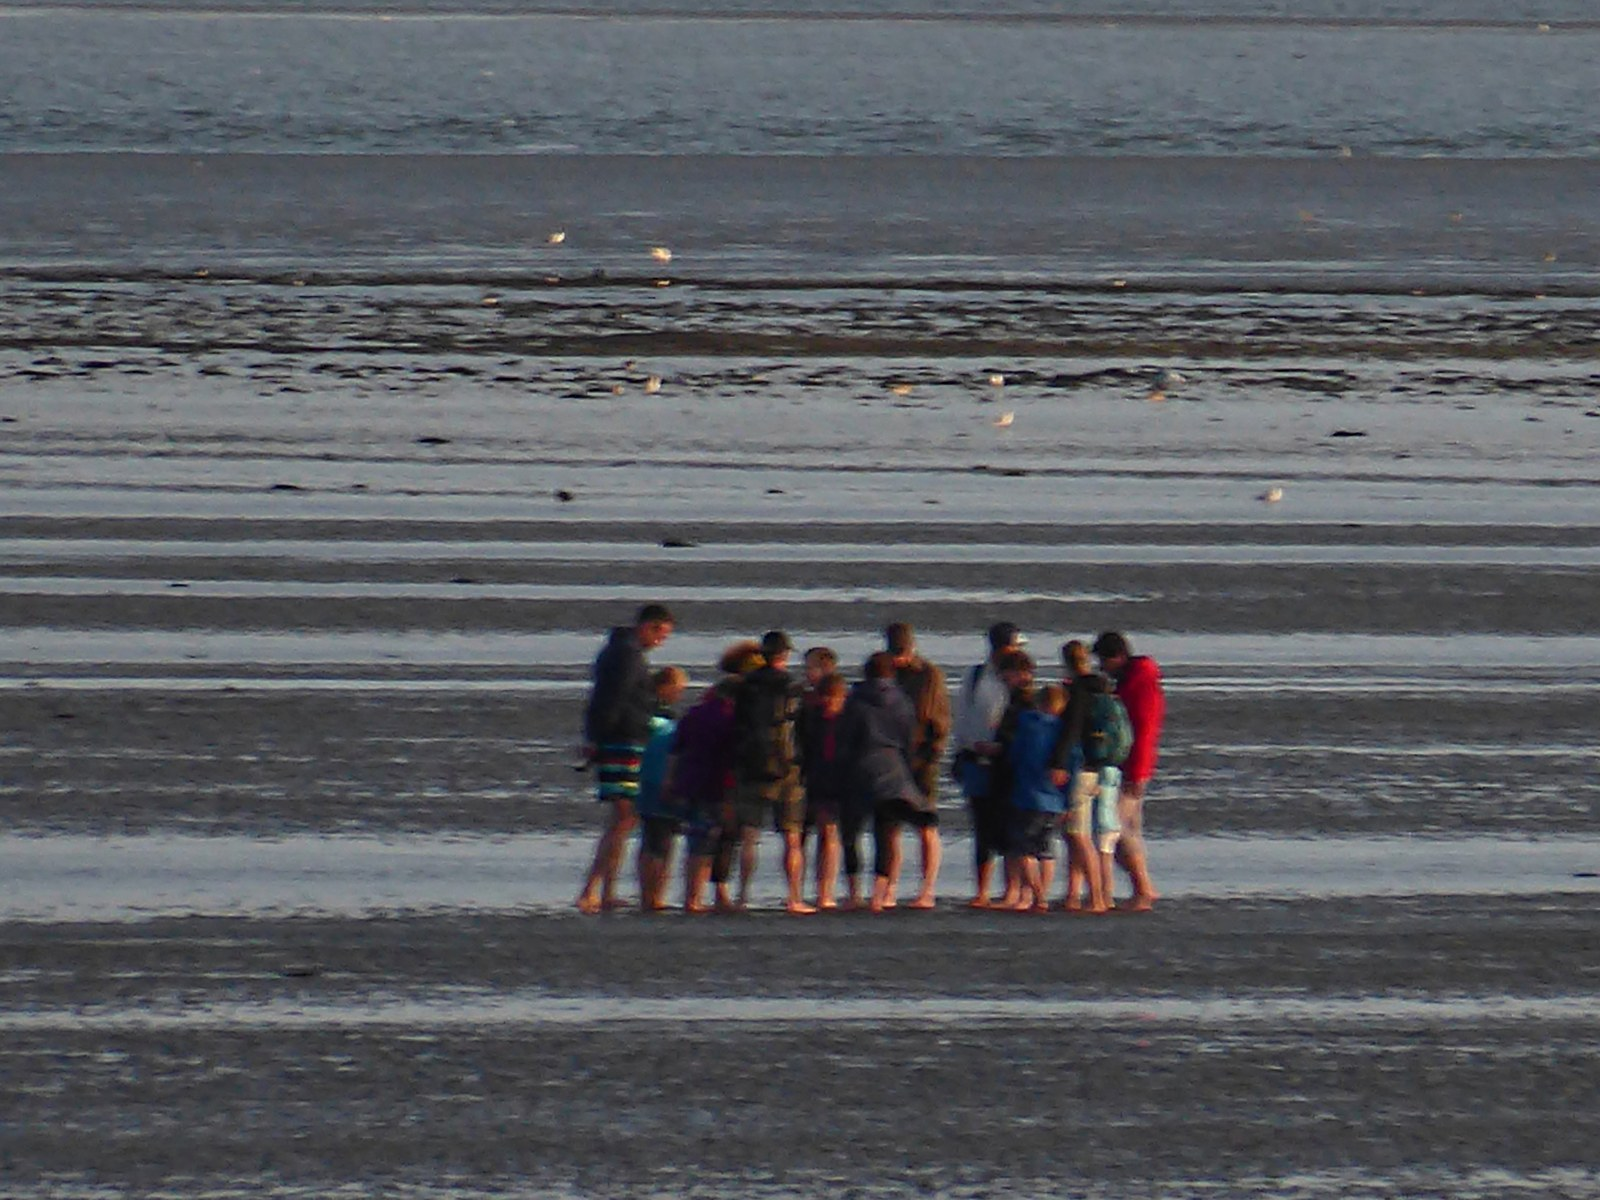
\includegraphics[width=0.49\textwidth]{figures/fig1_wadden_walk_cc0.jpg}\hfill
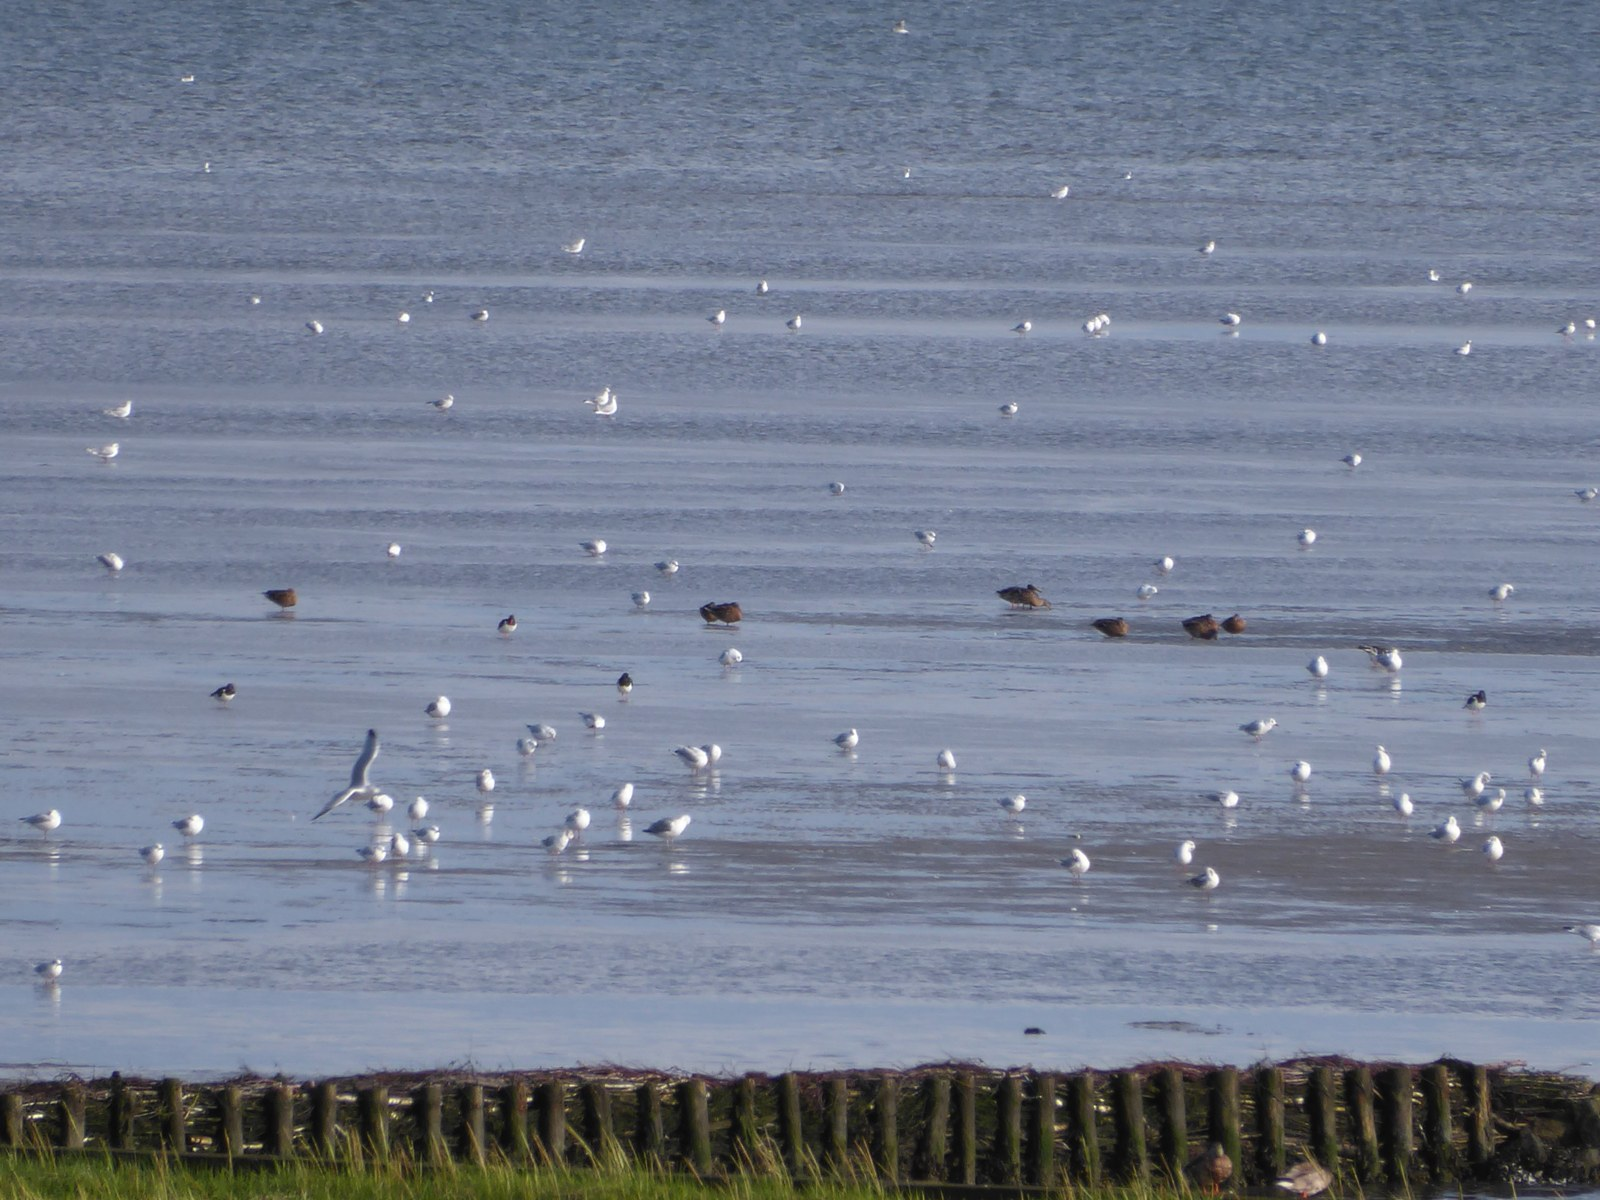
\includegraphics[width=0.49\textwidth]{figures/fig1_wadden_groyne_cc0.jpg}
\caption{Tidal flats at low water, seen from the ground (German Wadden
Sea, island of Wangerooge, August 2019). Left, a guided walk across the
flats south of the island, on sediment that the next high water will
cover. Right, the edge of the flat at a wooden groyne, with gulls and
waders feeding on the exposed mud. Photographs by Rhetos, Wikimedia
Commons, released under the CC0 1.0 public domain dedication.}
\label{fig:flats}
\end{figure}

Every one of these methods shares one input: the water level of each
scene, taken from a tide model or a tide gauge at a single point and
applied to the whole scene, or to a whole analysis cell
\citep{sagar2017,bishoptaylor2019ecss,bue2020,fitton2021,granadeiro2021,chen2025}.
Their authors state the consequence as a caveat. Sagar et al.~\cite{sagar2017}
acknowledge that ``using a single instantaneous tidal elevation value is no
doubt a simplification of reality''; Bishop-Taylor et al.~\cite{bishoptaylor2019ecss} expect
the assigned heights ``to rapidly decrease in accuracy with increasing
distance from a given modelling point'' and warn about lags ``on the
landward side of coastal wetlands \ldots or other environments such as
estuaries''; Bu\'e et al.~\cite{bue2020} attribute part of their $-0.51$~m bias on the
Tagus to the fact that ``different geographic areas at the Tagus estuary
have different tide height values for the same image acquisition time'';
Granadeiro et al.~\cite{granadeiro2021} detected phase differences of over one hour within a
single Sentinel-2 scene; and Chen and Wang~\cite{chen2025} reduced their mean absolute
error from 0.64 to 0.46~m simply by switching to a closer gauge. Working
with a shore-based radar, Bell et al.~\cite{bell2016} measured the effect directly: a
bias of 0.12~m within 0.75~km of the gauge growing to about 0.5~m farther
away. The accuracies these methods report against surveys, $\pm 0.39$~m on
tidal flats \citep{bishoptaylor2019ecss}, 0.57~m mean absolute difference
\citep{sagar2017}, 0.34~m with $-0.51$~m bias \citep{bue2020}, 0.24 to
0.59~m \citep{chen2025}, all carry this error inside them.

The error is not one a better global tide model can remove, because the
models themselves stop at the coast. The atlases that feed these pipelines,
FES2014 \citep{lyard2021}, EOT20 \citep{hartdavis2021} and the TPXO family
\citep{egbert2002}, usually through pyTMD \citep{sutterley2025,fitzpatrick2024},
are accurate to about 2~cm in
the open ocean but ``show large discrepancies between one another and
compared to in situ observations in the coastal region''
\citep{hartdavis2021}. EOT20 discards altimetry within 3 to 7~km of the
coastline, so it contains no observation inside an estuary; FES2014
resolves at best 1.5~km in estuaries and straits, never sees water
shallower than 10~m, and deliberately down-weights coastal gauges ``to
avoid drawing the solution to fit some very local tide features''
\citep{lyard2021}, while naming estuaries and deltas as an open problem.
Independent assessments find inter-model differences above 30~cm near
coasts and metre-level errors at individual gauges \citep{wang2025}, and
the best regional ensemble still leaves 0.29 to 0.36~m of error at
sheltered inlets \citep{bishoptaylor2026}, where a single model produced an
intertidal elevation model with ``visible sharp elevation discontinuities
and modelling artefacts'' that the same authors trace to the model being
out of phase with the real tide. Inside an estuary the tide is not the
ocean's tide: it arrives later the farther it travels up the channel, it
is amplified by convergence or damped by friction, and it is distorted by
shallow water \citep{friedrichs1994,savenije2005}. A level read at the
mouth, however good, is the wrong level
inland by an amount that grows with distance and is systematic across the
whole archive.

Two studies have looked to the imagery itself for the missing tidal
information. Granadeiro et al.~\cite{granadeiro2021} fit separate logistic curves to
rising- and ebbing-tide scenes and take, for each location, the lag that
reconciles the two elevations, obtaining cotidal lines over the Bijag\'os
archipelago within 6.6~min of the official values at five stations; but
the method returns one average lag per location, needs a reference site
with a known tide, was validated on an open archipelago rather than inside
an estuary, and its authors note that it cannot separate rising from
ebbing, spring from neap, or shallow from deep. Bishop-Taylor et al.~\cite{bishoptaylor2026}
rank ten global tide models by the correlation between each pixel's NDWI
and the modelled tide height, an approach that reads phase from the
imagery but, in their own words, could rank a model highly ``so long as it
correctly sorted satellite observations by tide height, even if it greatly
misrepresented tidal amplitude'', and they name estuarine amplification and
damping as the case it does not cover. Neither estimates the interior lag
with a statistical model of the pixel, states what a wet/dry archive can
and cannot identify, or tests a measured lag against what pure sampling
noise would produce.

This paper does those three things. We present MAREA, a method that treats
every intertidal pixel as a binary tide gauge and measures the phase lag of
the tide inside an estuary from the Sentinel-2 archive alone. The pixel
model is of the Rasch type, with scenes in the role of persons and pixels
in the role of items \citep{rasch1960,engelhard2021}. Per band of
along-channel distance from the mouth, the lag that best explains the
ten-year wet/dry record is the maximum of a profiled Bernoulli likelihood
in which each pixel's elevation and width are nuisance parameters fitted
under every candidate lag, in the manner of variable projection
\citep{golub1973,kaufman1975}; the mouth band is pinned to the ocean
model. We
show that this likelihood is invariant under a joint rescaling of tidal
gain, elevation and width, so that phase is identifiable from binary data
and gain and datum are not, and we build the adoption rule on that fact: a
lag is applied only where it leaves the range that replica archives with
the same pixels, clouds and dates but no interior tide produce, exceeds a
detection threshold and passes a physical veto. The boundary at the mouth
can be a global model, the nearest tide gauges or their consensus through
one interface, and gauges held out as judges never enter it. We validate
on four European estuaries with held-out gauges, on three of them against
the official Rijkswaterstaat bathymetry, and on the R\'ia de Villaviciosa
(Spain) against an RTK-GNSS survey, with the method of
Granadeiro et al.~\cite{granadeiro2021} reimplemented and run on the same pixels.
Section~\ref{sec:methods} describes the sites, the data, the method and
the validation design; Section~\ref{sec:results} presents the results and
discusses what the method can and cannot do; Section~\ref{sec:conclusions}
concludes. The code, the executed notebooks and the
negative results of the investigation are released with the paper.

\section{Methods}\label{sec:methods}

\subsection{Study sites and data}\label{sec:sites}

\subsubsection{Sites}

The method was developed on one estuary and its interior clock was tested
on four others (Fig.~\ref{fig:sites}, Table~\ref{tab:sites}). The development site is the R\'ia
de Villaviciosa, a 7~km drowned valley on the Cantabrian coast of northern
Spain with a narrow mouth, a single channel and mudflats on both banks.
Its ten-year Sentinel-2 archive at 10~m (1\,379 scenes) was the test bed
of every stage of the pipeline, and it holds the only field survey of the
study, an RTK-GNSS transect described below. No tide gauge exists inside
the r\'ia, so its boundary is the ocean model alone, and the surveyed
transect lies in the reach where the method measures no lag: Villaviciosa
therefore validates the elevation estimator, not the clock.

\begin{figure}[p]
\centering
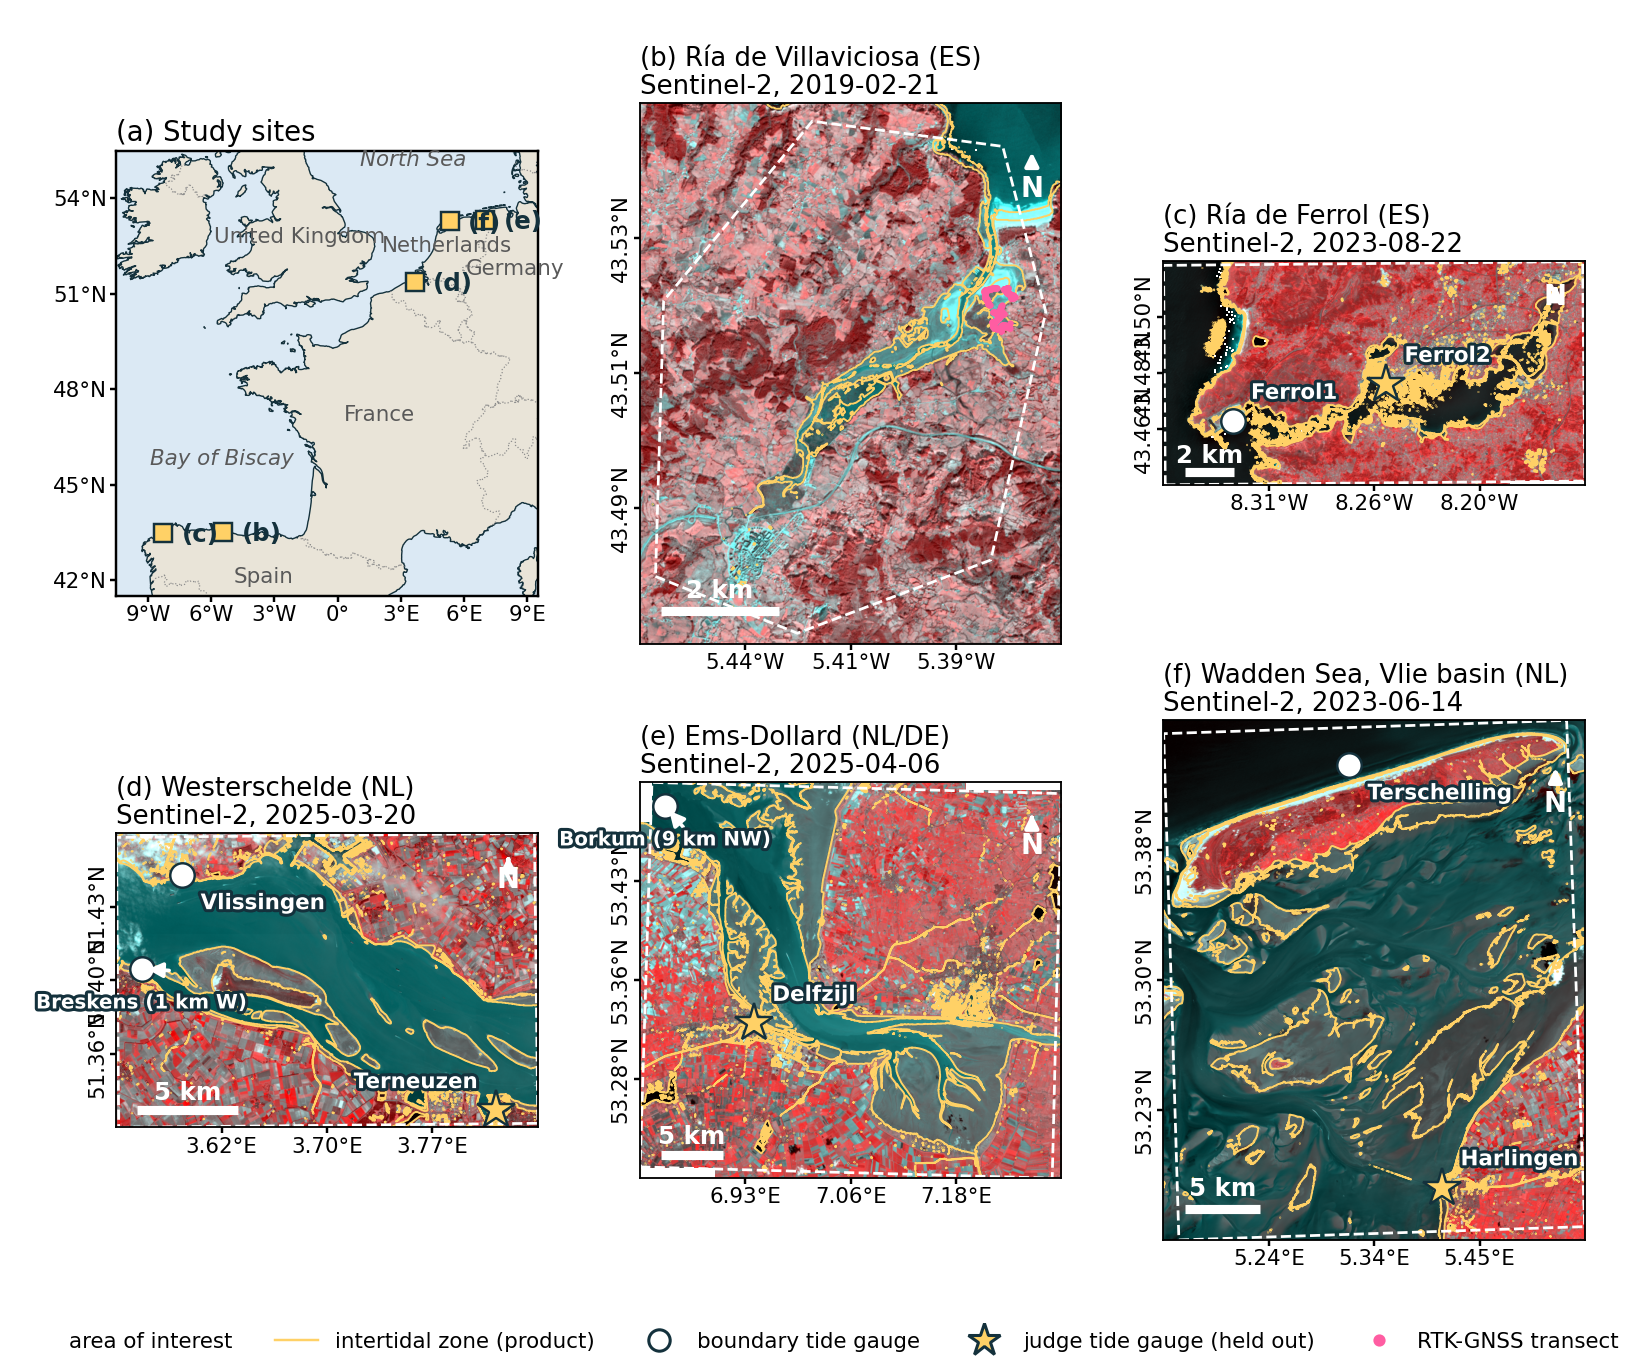
\includegraphics[width=\textwidth]{figures/fig_sites.png}
\caption{Study sites. (a) Location of the five sites on the Atlantic and
North Sea coasts of Europe (Natural Earth coastline). (b)--(f) Each site
on a clear low-water Sentinel-2 scene from its own datacube, shown as a
false-colour composite (near-infrared, green, green: water dark, exposed
sediment grey, vegetation red). The dashed line is the area of interest,
the yellow outline the intertidal zone retained by the product, circles
the tide gauges that feed the boundary and the star the gauge held out as
judge; a gauge outside the frame is marked at the nearest edge with its
distance. In (b) the magenta points are the development subset of the
RTK-GNSS survey. Scale bars and north arrows are per panel; the scene date
is in each title.}
\label{fig:sites}
\end{figure}

The four test sites were chosen by a single criterion: at least two tide
gauges on the same tidal axis, one at the mouth to feed the boundary and
one inside to judge, the latter never entering any fit. They span a range
of geometries. The R\'ia de Ferrol (Galicia) is a short, deep r\'ia with
small inner flats and the only Spanish gauge pair on one axis; it serves
as the negative control, a site where the tide should arrive almost
unchanged. The Westerschelde is the funnel-shaped mouth of the Scheldt
between Vlissingen and Terneuzen, with a dredged navigation channel and
wide sandbanks. The Ems-Dollard (Netherlands and Germany) is a 35~km
estuary whose inner basin, the Dollard, is a mudflat bay behind a
constricted channel. The Wadden site is the tidal basin behind the Vlie
inlet, between the barrier island of Terschelling and the port of
Harlingen, an open expanse of flats crossed by branching channels. The
three Dutch sites lie within the Rijkswaterstaat bathymetric survey, which
provides an independent elevation truth.

\begin{table}[t]
\centering
\caption{Study sites. Cubes are Sentinel-2 L2A datacubes at the stated
resolution; scenes are all acquisitions in the period, before cloud
screening. Intertidal pixels are those with water frequency between 0.10
and 0.90 and at least 30 clear observations. The judge's distance is the
geodesic distance through the water from the sea edge of the site.}
\label{tab:sites}
\footnotesize
\setlength{\tabcolsep}{4pt}
\resizebox{\textwidth}{!}{%
\begin{tabular}{@{}lrrrlll@{}}
\toprule
site & res. & period & scenes & intertidal px & boundary gauges & judge (km) \\
\midrule
R\'ia de Villaviciosa (ES)$^{a}$ & 10 m & 2016--25 & 1\,379 & --- & none (EOT20 only) & none \\
R\'ia de Ferrol (ES) & 10 m & 2023--25 & 461 & 103\,759 & Ferrol1 & Ferrol2 (10.1) \\
Westerschelde (NL)$^{b}$ & 20 m & 2023--25 & 464 & 73\,764 & Vlissingen, Breskens & Terneuzen (21.9) \\
Ems-Dollard (NL/DE)$^{b}$ & 20 m & 2023--25 & 462 & 477\,745 & Borkum & Delfzijl (24.4) \\
Wadden, Vlie basin (NL)$^{b}$ & 20 m & 2023--25 & 462 & 367\,076 & Terschelling & Harlingen (18.3) \\
\bottomrule
\multicolumn{7}{@{}l@{}}{$^{a}$ elevation truth: RTK-GNSS survey. $^{b}$ elevation truth: Rijkswaterstaat Vaklodingen.}
\end{tabular}}
\end{table}

\subsubsection{Sentinel-2 archive}

All imagery is Sentinel-2 Level-2A surface reflectance \citep{drusch2012},
processed with Sen2Cor \citep{mainknorn2017} and obtained from the
Copernicus Data Space Ecosystem through its openEO interface. For each
site one batch job retrieves every acquisition of the period, without any
cloud selection at download, into a single datacube of three layers per
scene: the green band B03, the near-infrared band B08, both at their
native 10~m, and the scene classification layer SCL. Every later stage
streams this cube; nothing is downloaded twice. Villaviciosa and Ferrol
are kept at 10~m; the three Dutch sites, an order of magnitude larger,
are resampled to 20~m at download. The water index is the NDWI of
McFeeters~\cite{mcfeeters1996}, $(\mathrm{B03}-\mathrm{B08})/(\mathrm{B03}+\mathrm{B08})$,
chosen over its short-wave infrared variant \citep{xu2006} because both
of its bands are native 10~m and because SWIR-based indices read wet
sediment as water on tidal flats
\citep{bishoptaylor2019waterline,bishoptaylor2026}. The acquisition
instant of every scene is taken from the catalogue metadata, not from the
nominal overpass time, because the difference reaches several minutes and
therefore several centimetres of tide.

\subsubsection{Tides}

The ocean boundary is the EOT20 global tide model \citep{hartdavis2021},
evaluated with pyTMD \citep{sutterley2025} at a fixed point in the mouth
channel of each site at the exact acquisition instant of each scene. Tide
gauge records come from the IOC Sea Level Station Monitoring Facility
\citep{ioc2026} at minute-scale sampling for 2023--2025. They are cleaned
before use: isolated spikes are removed with a rolling median (61~min
window, 0.75~m tolerance), values beyond 6~m and residuals from a
harmonic fit beyond 2.5~m are discarded, the record is demeaned, and gaps
longer than one hour are left as gaps rather than bridged; the Vlissingen
record, for instance, is missing for eighteen months of the period. A
boundary can then be the model alone, the $N$ nearest gauges blended with
inverse-square-distance weights, or the consensus of the two, the plain
mean of model and gauge blend; which one is used is stated with every
result, and the judge gauge of a site is excluded from its boundary in
every case.

\subsubsection{Elevation truth}

Two independent sources of elevation are used. For the Dutch sites, the
Vaklodingen of Rijkswaterstaat \citep{rws_vaklodingen}, the national
bathymetric and topographic grids of the coastal waters, surveyed by
echo-sounding and airborne laser altimetry on 20~m cells relative to the
NAP datum in the Dutch RD projection; 32 sheets cover the three sites,
each with its own survey year, the German part of the Dollard being last
surveyed in 2020. For Villaviciosa, an RTK-GNSS survey of the flats: 361
fixed solutions with a nominal precision of 1.3~cm, walked along a
0.75~km transect at the lowest spring tide of the month. Before any
elevation product existed, 35\,\% of the surveyed pixel blocks were
sealed as a reserved set, locked by a runtime guard and opened once for a
verdict recorded in the repository; all numbers in this paper use the
development subset. The 5~m national LiDAR was examined as a third source
and rejected: over the intertidal mask it records the water surface at
flight time rather than the bed. All three truths are in datums other
than the tide model's, so every comparison removes the median offset
between product and truth and reports it separately
(Section~\ref{sec:validation}).

% Draft of Sections 2.2-2.5 (Methods). Body text only; to be pasted into
% main.tex in place of the four "(to be written)" placeholders.
% Sources: docs/METHOD.md, docs/one_pixel_marea_example.md,
% docs/tide_adjustment_comparison.md (1, 5), docs/prior_art_granadeiro.md,
% pyintertidal/marea.py, pyintertidal/tide_estimators.py,
% pyintertidal/elevation.py, configs/m2.yaml, experiments/sota_granadeiro.py,
% experiments/e0_escalda_prep.py.

\subsection{The pixel model and the elevation inversion}\label{sec:pixel}

For a shoreline pixel with flooded fraction $f$, linear mixing of the
McFeeters water index~\cite{mcfeeters1996} gives
\begin{equation}\label{eq:mix}
\mathrm{NDWI} = (1-f)\,\mathrm{NDWI}_{\mathrm{dry}} + f\,\mathrm{NDWI}_{\mathrm{wet}}
= a + b\,f ,
\end{equation}
where the dry level $a$ and the dry-to-wet jump $b$ are fitted per
pixel, which normalises albedo between pixels. At water level $h$,
$f(h) = \Pr(\text{internal elevation} \le h)$ is the cumulative
distribution of the pixel's relief, assumed Gaussian with mean $z$, its
median elevation, and spread $\sigma$, its roughness:
\begin{equation}\label{eq:pixel}
\mathrm{NDWI}(h) = a + b\,\Phi\!\left(\frac{h - z}{\sigma}\right),
\end{equation}
with $\Phi(u) = (2\pi)^{-1/2}\int_{-\infty}^{u} e^{-v^{2}/2}\,\mathrm{d}v$
the standard normal distribution function; the midpoint $h = z$ is the
elevation. Eq.~\eqref{eq:pixel} is the probit ogive of
quantal-response analysis \cite{bliss1934,finney1947}, the Gaussian
counterpart of the per-pixel methods' logistic \cite{berkson1944}. The
fitted $\sigma$ also absorbs the water-level error of each scene.

The inversion (\texttt{invert\_series}) fits Eq.~\eqref{eq:pixel} to
each pixel's clear observations by least squares: for each candidate
$(z, \sigma)$ the linear $(a, b)$ is solved in closed form, $z$ runs
over 50 points between the lowest and highest level of the series,
$\sigma$ over the archive's eight relief atoms (0.03, 0.06, 0.10, 0.15,
0.22, 0.32, 0.45 and 0.65~m), and the pair with the smallest residual is
kept. A pixel is left blank with fewer than 8 clear observations, a
contrast $b$ outside $(0.15, 2.5)$ or a dry level $|a| \ge 2.5$.

A scene is kept if at most 10\,\% of the transition zone is cloudy; an
observation is used only where Sen2Cor reads vegetation, bare ground or
water (the campaign extraction also admits unclassified). The wet/dry
label is $\mathrm{NDWI} > 0$: Otsu's threshold \cite{otsu1979} on the
twelve clearest development-site scenes lands at $+0.25$, the top of its
allowed range; zero is preferred because turbid estuarine water reads
lower than clear water. The intertidal zone is delimited by water
frequency, the wet fraction of a pixel's clear observations. A
three-class Otsu split of the transition pixels separates ground, flat
and channel, with valleys at 0.21 and 0.66 in Villaviciosa, and
confirms that the archive holds three populations; but the flats reach
far into the rarely wet class: of the 181 intertidal pixels the
development RTK survey covers, only 79 lie inside the Otsu window
against 130 inside 0.05--0.95. The window is therefore set by what the
inversion
can resolve, a pixel with enough clear observations on both sides of
its transition, and opened to 0.05--0.95. The four test-site products
use the fixed window and minimum count of Section~\ref{sec:sites}. Elevations are fitted within an epoch,
2023--2025 for the products of Section~\ref{sec:results}.

\subsection{The interior clock}\label{sec:clock}

The interior tide is measured per band of along-channel distance $s$
from the mouth: $s$ is the geodesic distance, the minimum-cost
eight-connected path over the permanent-water and intertidal masks
times the pixel size, from the permanent-water pixels (water frequency
at least 0.90) on the image border on the sides declared as sea.
Intertidal pixels are split into 3-km bands along $s$; a band with fewer
than 500 pixels is merged with the next. Each band sits at the median
$s$ of its pixels, and at most 1\,200 of them, drawn at random with a
fixed seed, enter the likelihood.

% fig:method removed from the paper (its panels are in the pipeline and
% likelihood figures); experiments/paper_fig_method.py is kept.


Each observation is reduced to its binary label $y_{pt} \in \{0,1\}$ and
the amplitudes of Eq.~\eqref{eq:pixel} are fixed at 0 and 1, leaving two
parameters per pixel: a Rasch-type model \cite{rasch1960,engelhard2021}
(scenes as persons, pixels as items). Under a candidate clock $\tau_k$
for band $k$ the level at scene $t$ is $h(t-\tau_k)$, pixel $p$ is wet
with probability $P_{pt} = \Phi\big((h(t-\tau_k) - z_p)/\sigma_p\big)$,
and the profiled Bernoulli log-likelihood of the band is
\begin{equation}\label{eq:profile}
\ell_k(\tau_k) = \sum_{p \in k}\; \max_{z_p,\,\sigma_p}\; \sum_{t}
\Big[\, y_{pt}\log P_{pt} + (1-y_{pt})\log(1-P_{pt}) \Big],
\end{equation}
where $t$ runs over the pixel's clear scenes. The inner maximum is the
profiling of variable projection \cite{golub1973,kaufman1975}: every
pixel re-fits its own $(z_p, \sigma_p)$ under each clock, so clocks are
decided only by what terrain cannot absorb, the reordering of the tide
across dates (Fig.~\ref{fig:likelihood}). The grid is 60 points of $z_p$
over the boundary's tidal range plus 0.3~m on either side, about 8~cm
apart, and, in the product, the six interior relief atoms, 0.06 to
0.45~m, for $\sigma_p$; probabilities are clipped at $10^{-4}$, and a
pixel needs at least six clear scenes.

The boundary is evaluated once at every acquisition instant shifted by
the sixteen values $-45, -30, \ldots, 180$~min of the shift bank, and
$h(t-\tau)$ is interpolated linearly between them. The mouth band is
pinned at $\tau_0 = 0$. The free parameters are the increments between
successive bands, $\tau_k = \sum_{j \le k} \delta_j$ with every
$\delta_j \ge 0$, so the profile is monotone non-decreasing inland. The
negative of Eq.~\eqref{eq:profile}, summed over bands and normalised per
observation, is minimised with L-BFGS-B \cite{byrd1995} in SciPy
\cite{virtanen2020}, the increments in hours, bounded between 0 and
$+180$~min and started at zero.

\begin{figure*}[t]
\centering
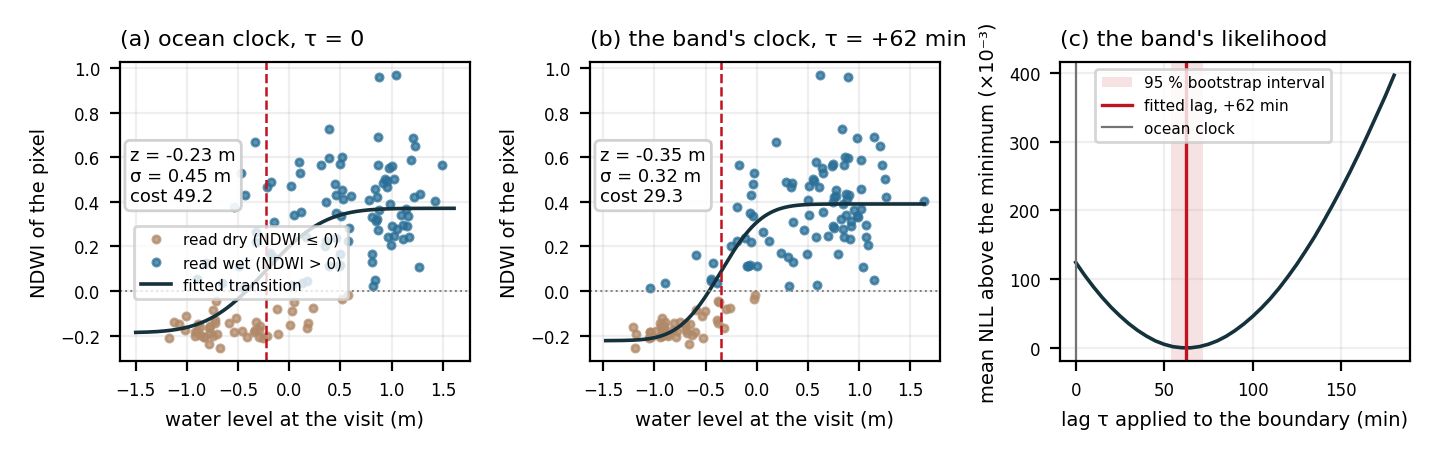
\includegraphics[width=0.86\textwidth]{fig_likelihood.png}
\caption{What the clock does to the likelihood, on the Ems-Dollard band
containing the Delfzijl gauge. (a) One pixel of the band on the ocean
clock: its NDWI at each visit against the water level at the mouth,
coloured by the reading (wet above 0, dry below), and the transition
$a + b\,\Phi((h - z)/\sigma)$ with the $(z, \sigma)$ profiled by the
binary likelihood; wet and dry readings overlap over a wide range of
levels. (b) The same pixel on the band's clock: the readings separate,
the transition sharpens and the pixel's negative log-likelihood (cost)
falls. (c) The band's profiled
negative log-likelihood against the lag, relative to its minimum, with
the fitted lag, its 95\,\% bootstrap interval and the ocean clock.}
\label{fig:likelihood}
\end{figure*}

\subsection{Identifiability and adoption}\label{sec:adoption}

The interior tide may also be amplified or damped: with a gain $\alpha$
and a datum shift, $h_{\mathrm{int}}(t) = \alpha\,h(t-\tau) + \mathrm{datum}$.
Binary data cannot read $\alpha$: with $P = \Phi\big((\alpha h - z)/\sigma\big)$,
multiplying $\alpha$, $z$ and $\sigma$ by one constant $c$ gives
\begin{equation}\label{eq:affine}
\frac{(c\alpha)\,h - (cz)}{c\sigma} = \frac{\alpha h - z}{\sigma},
\end{equation}
so the likelihood is unchanged, and a datum shift is absorbed by $z$.
Only the phase survives, so it is measured from the imagery; gain and
datum come from the boundary. The check is executable: with a gain of
1.0--1.3 planted in the simulator, the negative log-likelihood profile
in $\alpha$, with $(z, \sigma)$ profiled on grids scaling with $\alpha$,
must be flat.

Each band lag carries a scene-bootstrap interval: the scenes are
resampled with replacement thirty times, the profile refitted on each,
and the 2.5th and 97.5th percentiles of the thirty $\tau_k$ are its
95\,\% confidence interval; an interval containing zero means the lag is
not distinguishable from none. No threshold is applied and no lag
discarded; the interval says which values carry information. On replica
archives with the pixels, cloud masks and acquisition instants of a real
site but a uniform tide with no interior lag, the estimator returns lags
of the order of ten minutes; the experiments are released with the code.

Each pixel receives the band profile smoothed along $s$ with a Gaussian
kernel of the band length, anchored at $\tau = 0$ at the mouth and kept
monotone, evaluated at the pixel's own distance and rounded to the
minute. The inversion of Section~\ref{sec:pixel} is then run once with
the boundary evaluated at the exactly shifted instants $t - \tau$, not
the bank's 15-min interpolation, and the $z$ grid spanning the unshifted
boundary range everywhere. The product stores the band lags, their
intervals and the lag every pixel received.

\subsection{The comparison method}\label{sec:granadeiro}

The elevation maps are compared with those of the published method of
Granadeiro et al.~\cite{granadeiro2021}, which fits a logistic with
four parameters to standardised near-infrared reflectance against water
height
per pixel, the inflection being the elevation, and reads a tidal-stage
lag per pixel from the disagreement between its rising and ebbing fits,
extended over the flat by a thin-plate spline. It was reimplemented from
the paper, not their code, with SciPy \cite{virtanen2020} for the fits,
and run on the same pixels, scenes and boundary as MAREA; the
reimplementation and its declared substitutions are released with the
code.


% Validation (2.6) and the whole of Section 3 (results skeleton); the
% numbers in its tables are refilled from the notebook outputs after each
% re-execution of the pipeline.
% Validation subsection (2.6) and Section 3, \input by main.tex.
% Every number must trace to the CSVs the pipeline notebooks write
% (tide_boundary_comparison_<site>.ipynb sections 10/10b,
% intertidal_topography_villaviciosa.ipynb sections 9a/9b); the scripts
% experiments/v4_lag_external.py, v5_rtk_onsite.py and v6_lidar_external.py
% only assemble them into results/*.json and the paper figures.
% Convention: "MAREA's lag at the inner gauge" is the smoothed band profile
% evaluated at the gauge's distance from the mouth, i.e. what a pixel there
% receives; the band that contains the gauge and its 95 % interval are
% given beside it. The comparison method's lag is not scored against gauges.
% Runs of 2026-09-23 (fixed-band product): Ferrol, Westerschelde, Ems and
% Wadden done; Villaviciosa (RTK, LiDAR) pending -> \ldots.

\subsection{Validation}\label{sec:validation}

The method yields two quantities, the lag of each band and the elevation
of each pixel, each validated on site, in the R\'ia de Villaviciosa, and
externally, against tide-gauge records and surveys made by others
(Table~\ref{tab:validation}). The lag blocks ask whether the measured
lag is real and whether applying it improves the level assigned inside
the estuary; the elevation blocks set both maps against independent
surveys. Nothing that judges a result enters a fit.

\begin{table*}[t]
\centering
\caption{The four validation blocks: what is validated, against what,
where, and with which metric.}
\label{tab:validation}
\footnotesize
\setlength{\tabcolsep}{5pt}
\resizebox{\textwidth}{!}{%
\begin{tabular}{@{}llll@{}}
\toprule
block & reference & sites & metric \\
\midrule
lag, on site & pressure sensors along the r\'ia & Villaviciosa & lag in reaching the same level (min); \\
 & (campaign pending) & & same-instant level difference (m) \\
lag, external & gauge pair: mouth and inner (judge) & Ferrol, Westerschelde, & gauge-pair lag vs.\ lag applied (min); \\
 & & Ems-Dollard, Wadden & RMSE of the level at the judge, without \\
 & & & and with the lag (m) \\
elevation, on site & RTK-GNSS survey, development split & Villaviciosa & RMSE, slope $b$, $r$ of each map on the \\
 & & & survey (Eq.~\ref{eq:metrics}); transect profile \\
elevation, external & IGN LiDAR DTM; Vaklodingen & Spanish sites; Dutch sites & RMSE, slope $b$, $r$ (Eq.~\ref{eq:metrics}), \\
 & & & by band for the Vaklodingen \\
\bottomrule
\end{tabular}}
\end{table*}

\subsubsection{Metrics and the datum}

Lags are compared in minutes: the gauge-pair lag is the mean over
paired tidal cycles $c$ of $t^{\mathrm{in}}_c - t^{\mathrm{mouth}}_c$,
the instants at which the inner and the mouth record cross the same
level on the same limb, and it is set against the lag MAREA applies at
the inner gauge. The effect of a lag on the water level is the RMSE
between the level a product predicts there, the boundary $h_B$ read
$\tau$ minutes earlier, and the level $h^{\mathrm{in}}$ the gauge
recorded, the median of the difference (the datum) removed:
\begin{align}
\mathrm{RMSE}_h &= \sqrt{\frac{1}{N}\sum_{t}\big(d(t) - \operatorname{median}\,d\big)^{2}}, \nonumber \\
d(t) &= h_B(t - \tau) - h^{\mathrm{in}}(t),
\label{eq:judge}
\end{align}
over the $N$ ten-minute samples of 2023--2025. Elevations are compared
with Eq.~\eqref{eq:metrics}. Products are on the datum of the tide model at
the mouth, the mean sea level of EOT20 \cite{hartdavis2021}; each truth
is on its own: NAP for the Vaklodingen \cite{rws_vaklodingen}, the
ellipsoid for the RTK-GNSS survey, orthometric heights for the LiDAR. No
method can see the constant between the two, so every comparison removes
it and reports it as the bias. On the $n$ samples where product $z$ and
truth $z^{\mathrm{t}}$ are both finite, each series is centred on its own
median, $y_i = z_i - \operatorname{median}(z)$ and
$x_i = z^{\mathrm{t}}_i - \operatorname{median}(z^{\mathrm{t}})$, and
\begin{align}
\mathrm{RMSE} &= \sqrt{\frac{1}{n}\sum_{i=1}^{n}(y_i - x_i)^2}, \qquad
b = \frac{\sum_i (x_i-\bar x)(y_i-\bar y)}{\sum_i (x_i-\bar x)^2}, \nonumber \\
r &= \frac{\sum_i (x_i-\bar x)(y_i-\bar y)}
         {\sqrt{\sum_i (x_i-\bar x)^2\,\sum_i (y_i-\bar y)^2}},
\label{eq:metrics}
\end{align}
with the truth on the abscissa: the slope $b$ says whether the map
reproduces the relief (1) or compresses it (below 1), $r$ how much of it
the map explains. Only truth within the range of scene levels, widened
by $\pm 0.25$~m, is scored: no waterline method can represent a channel
bed at $-8$~m beside a flat. A $5 \times 5$ thinning of the grid, one
pixel per 100~m block, changed no ranking.

\subsubsection{The interior lag on site: pressure sensors along the r\'ia}

The R\'ia de Villaviciosa has no interior tide gauge, so its lag will be
measured directly: absolute pressure sensors at three to four stations,
submerged through the lowest spring low water, with a barometer on land,
over 29 days at 1 to 5~min. Level follows
$h = z_s + (p - p_{\mathrm{atm}})/(\rho g)$, with $\rho = 1025$~kg\,m$^{-3}$
and $z_s$ the sensor elevation from RTK-GNSS. Each station is then
scored against the mouth as the gauge pairs below. The campaign is
pending.

\subsubsection{The interior lag against gauge pairs}

Four estuaries have a gauge near the mouth and another inside, the judge
of Section~\ref{sec:sites}: Ferrol1 and Ferrol2, Vlissingen and
Terneuzen, Borkum and Delfzijl, Terschelling Noordzee and Harlingen. Two quantities need
only the two records \cite{ioc2026}, 2023--2025, 10-min grid, demeaned,
gaps over one hour left open. The first is the lag in reaching the same
level: crossings of the 25th, 50th and 75th percentile of the mouth's
level are interpolated between samples and paired with the nearest inner
crossing within three hours; their mean difference over paired cycles,
and per limb, is the gauge-pair lag. It is compared with the lag MAREA
applies at the gauge's distance and with the 95\,\% bootstrap interval of
the band containing the inner gauge, measured from band 0, which holds
the mouth gauge (\emph{no delay}: 0 everywhere). The second is the
same-instant level difference, inner minus mouth: its RMS and mean are
the error of the uniform level every published method assumes. The third
is the level predicted at the inner gauge from the mouth boundary read
$\tau$ minutes earlier, with $\tau = 0$ and with MAREA's lag there,
scored on the gauge's record as the median-centred RMSE of
Eq.~\eqref{eq:metrics}. Nothing was fitted on the inner gauge, so the
whole record is the test. The comparison method's lag, per pixel over
the flats, reaches no gauge and is scored only through its elevations.

\subsubsection{Elevation on site: the RTK-GNSS survey}

In Villaviciosa the maps are scored on the development subset of the
RTK-GNSS survey of Section~\ref{sec:sites}: 35\,\% of its 150~m blocks,
drawn once with a fixed seed and sealed before any elevation product
existed, released by a runtime guard only to the verdict script. The two
maps share record, epoch (2023--2025) and boundary (EOT20 at the mouth):
\emph{MAREA}, our inversion with the smoothed band profile at each
pixel's distance, and \emph{Granadeiro}, the method of
Section~\ref{sec:granadeiro} with its own lag map. Both are scored with
Eq.~\eqref{eq:metrics} and drawn with the survey along a straight
stretch of the walked route.

\subsubsection{Elevation external: the national LiDAR and the Vaklodingen}

At the Spanish sites, Villaviciosa and Ferrol, the reference is the 5~m
LiDAR DTM of the Instituto Geogr\'afico Nacional (PNOA),
% TODO: add a bib entry for the IGN MDT05 / PNOA-LiDAR product
resampled bilinearly onto the product grid; at the Dutch sites, the
Rijkswaterstaat Vaklodingen \cite{rws_vaklodingen}, yearly bathymetry
and intertidal topography on a 20~m grid (NAP), each pixel taking its
nearest cell's latest survey of 2019--2025. Both maps are scored with
Eq.~\eqref{eq:metrics} on the intertidal pixels each resolves and on
those both resolve, the Vaklodingen also by band of distance from the
mouth. A LiDAR flown at high water records the water surface over the
flats, so each LiDAR score comes with the water share of its truth: the
share of intertidal cells within 5~cm of the modal value.

\section{Results and discussion}\label{sec:results}

\subsection{The interior lag against the gauge pairs}\label{sec:res_lag}

\begin{table*}[t]
\centering
\caption{The interior lag against the gauge pairs, 2023--2025. Lag between
the mouth gauge and the inner gauge in reaching the same level (mean over
paired cycles and limbs, positive: the inner gauge is later); lag MAREA
applies at the inner gauge, with the 95\,\% bootstrap interval of its
band; RMS difference between the two gauge records at the same instant,
the error of copying the mouth gauge inland; and the RMSE of the level
predicted at the inner gauge from the boundary the products use (the
consensus of EOT20 and the mouth gauge), without and with the lag.
% NUMBERS: lag_pair_metrics.csv and judge_metrics.csv of each site's
% comparison notebook, run of 2026-09-23.
}
\label{tab:lag_external}
\footnotesize
\setlength{\tabcolsep}{6pt}
\begin{tabular}{@{}lrrrr@{}}
\toprule
 & lag between & lag applied & inner vs.\ mouth gauge, & level at the inner gauge from \\
site (inner gauge, km from mouth) & gauges (min) & by MAREA (min) & same instant, RMS (m) & the boundary (m): no lag $\to$ MAREA \\
\midrule
Ferrol (Ferrol2, 10.1) & $+4$ & $0$ $[0, +2]$ & 0.10 & $0.112 \to 0.112$ \\
Westerschelde (Terneuzen, 21.9) & $+19$ & $+7$ $[+4, +17]$ & 0.28 & $0.356 \to 0.311$ \\
Ems-Dollard (Delfzijl, 24.4) & $+51$ & $+63$ $[+54, +72]$ & 0.50 & $0.620 \to 0.358$ \\
Wadden, Vlie (Harlingen, 18.3) & $+88$ & $+129$ $[+123, +138]$ & 0.53 & $0.562 \to 0.303$ \\
\bottomrule
\end{tabular}
\end{table*}

% figure fig:lag_external is placed after the bibliography (main.tex)


% Numbers: lag_pair_metrics.csv and judge_metrics.csv of each site (run of
% 2026-09-23).
The gauge pairs order the sites as the archive does
(Table~\ref{tab:lag_external}, Fig.~\ref{fig:lag_external}). In Ferrol
the inner gauge lags the mouth by 4~min and one level for the whole
r\'ia errs by 0.10~m RMS; MAREA measures 0~min there, interval 0 to
$+2$, and the level error stays at 0.112~m. In the Westerschelde the
gauges are 19~min apart on both limbs; MAREA applies $+7$~min at
Terneuzen, the band's interval reaching $+17$, and the error falls from
0.356 to 0.311~m. In the Ems-Dollard the lag is 51~min, 41 rising and 61
falling; MAREA applies $+63$~min at Delfzijl, inside its interval of
$+54$ to $+72$, and the error falls from 0.620 to 0.358~m, by 42\,\%. In
the Vlie basin the gauges are 88~min apart, 91 rising and 85 falling;
MAREA applies $+129$~min at Harlingen, interval $+123$ to $+138$, 41~min
beyond the gauges, and the error still falls from 0.562 to 0.303~m, by
46\,\%. Two columns of Table~\ref{tab:lag_external} differ in kind: the
same-instant difference sets the two gauge records against each other,
whereas the level error is that of the boundary the products read, the
consensus of EOT20 and the mouth gauge, which adds the model's error to
the uniform-level assumption; hence the boundary without a lag (0.620~m
in the Ems-Dollard) is worse than the mouth gauge copied inland
(0.50~m), and MAREA with the lag (0.358~m) beats either. Where an
interior tide exists the archive measures it; where none exists it
applies the few minutes its intervals declare, at a cost of centimetres
at most.

\subsection{Elevation against the RTK survey}\label{sec:res_rtk}

\begin{table}[t]
\centering
\caption{Elevation against the RTK-GNSS survey, Villaviciosa development
subset, 2023--2025, EOT20 boundary. $n$: surveyed points the map
resolves; RMSE, slope $b$ and $r$ as in Eq.~\eqref{eq:metrics}, RTK on
the abscissa; bias: the datum offset, ellipsoidal heights against the
tide-model datum, removed before scoring.
% NUMBERS: products_marea/rtk_onsite_metrics.csv (Villaviciosa notebook,
% section 9a), run pending.
}
\label{tab:rtk}
\footnotesize
\begin{tabular}{@{}lrrrrr@{}}
\toprule
method & $n$ & RMSE (m) & $b$ & $r$ & bias (m) \\
\midrule
MAREA & 194 & 0.193 & 0.72 & 0.86 & $-52.8$ \\
Granadeiro & 163 & 0.275 & 0.39 & 0.63 & $-53.3$ \\
\bottomrule
\end{tabular}
\end{table}

% figure fig:rtk_onsite is placed after the bibliography (main.tex)



% Numbers: products_marea/rtk_onsite_metrics.csv (section 9a of the
% Villaviciosa notebook; experiments/v5_rtk_onsite.py runs the same code).
On the 194 surveyed points it resolves, MAREA reaches 0.193~m RMSE with
slope 0.72 and $r = 0.86$; the Granadeiro map reaches 0.275~m with
slope 0.39 and $r = 0.63$ on 163 points (Table~\ref{tab:rtk},
Fig.~\ref{fig:rtk_onsite}a,b). Along a straight 192-m stretch of the
walked route
(Fig.~\ref{fig:rtk_onsite}c--e) the MAREA profile follows the survey
within the pixel size, including the fall at its inland end, where the
Granadeiro profile stays flat. The lag applied on the surveyed pixels is
5~min in median and 16 at most, so Villaviciosa tests the estimator
more than the clock.

\subsection{Elevation against the external references}\label{sec:res_lidar}

\begin{figure*}[t]
\centering
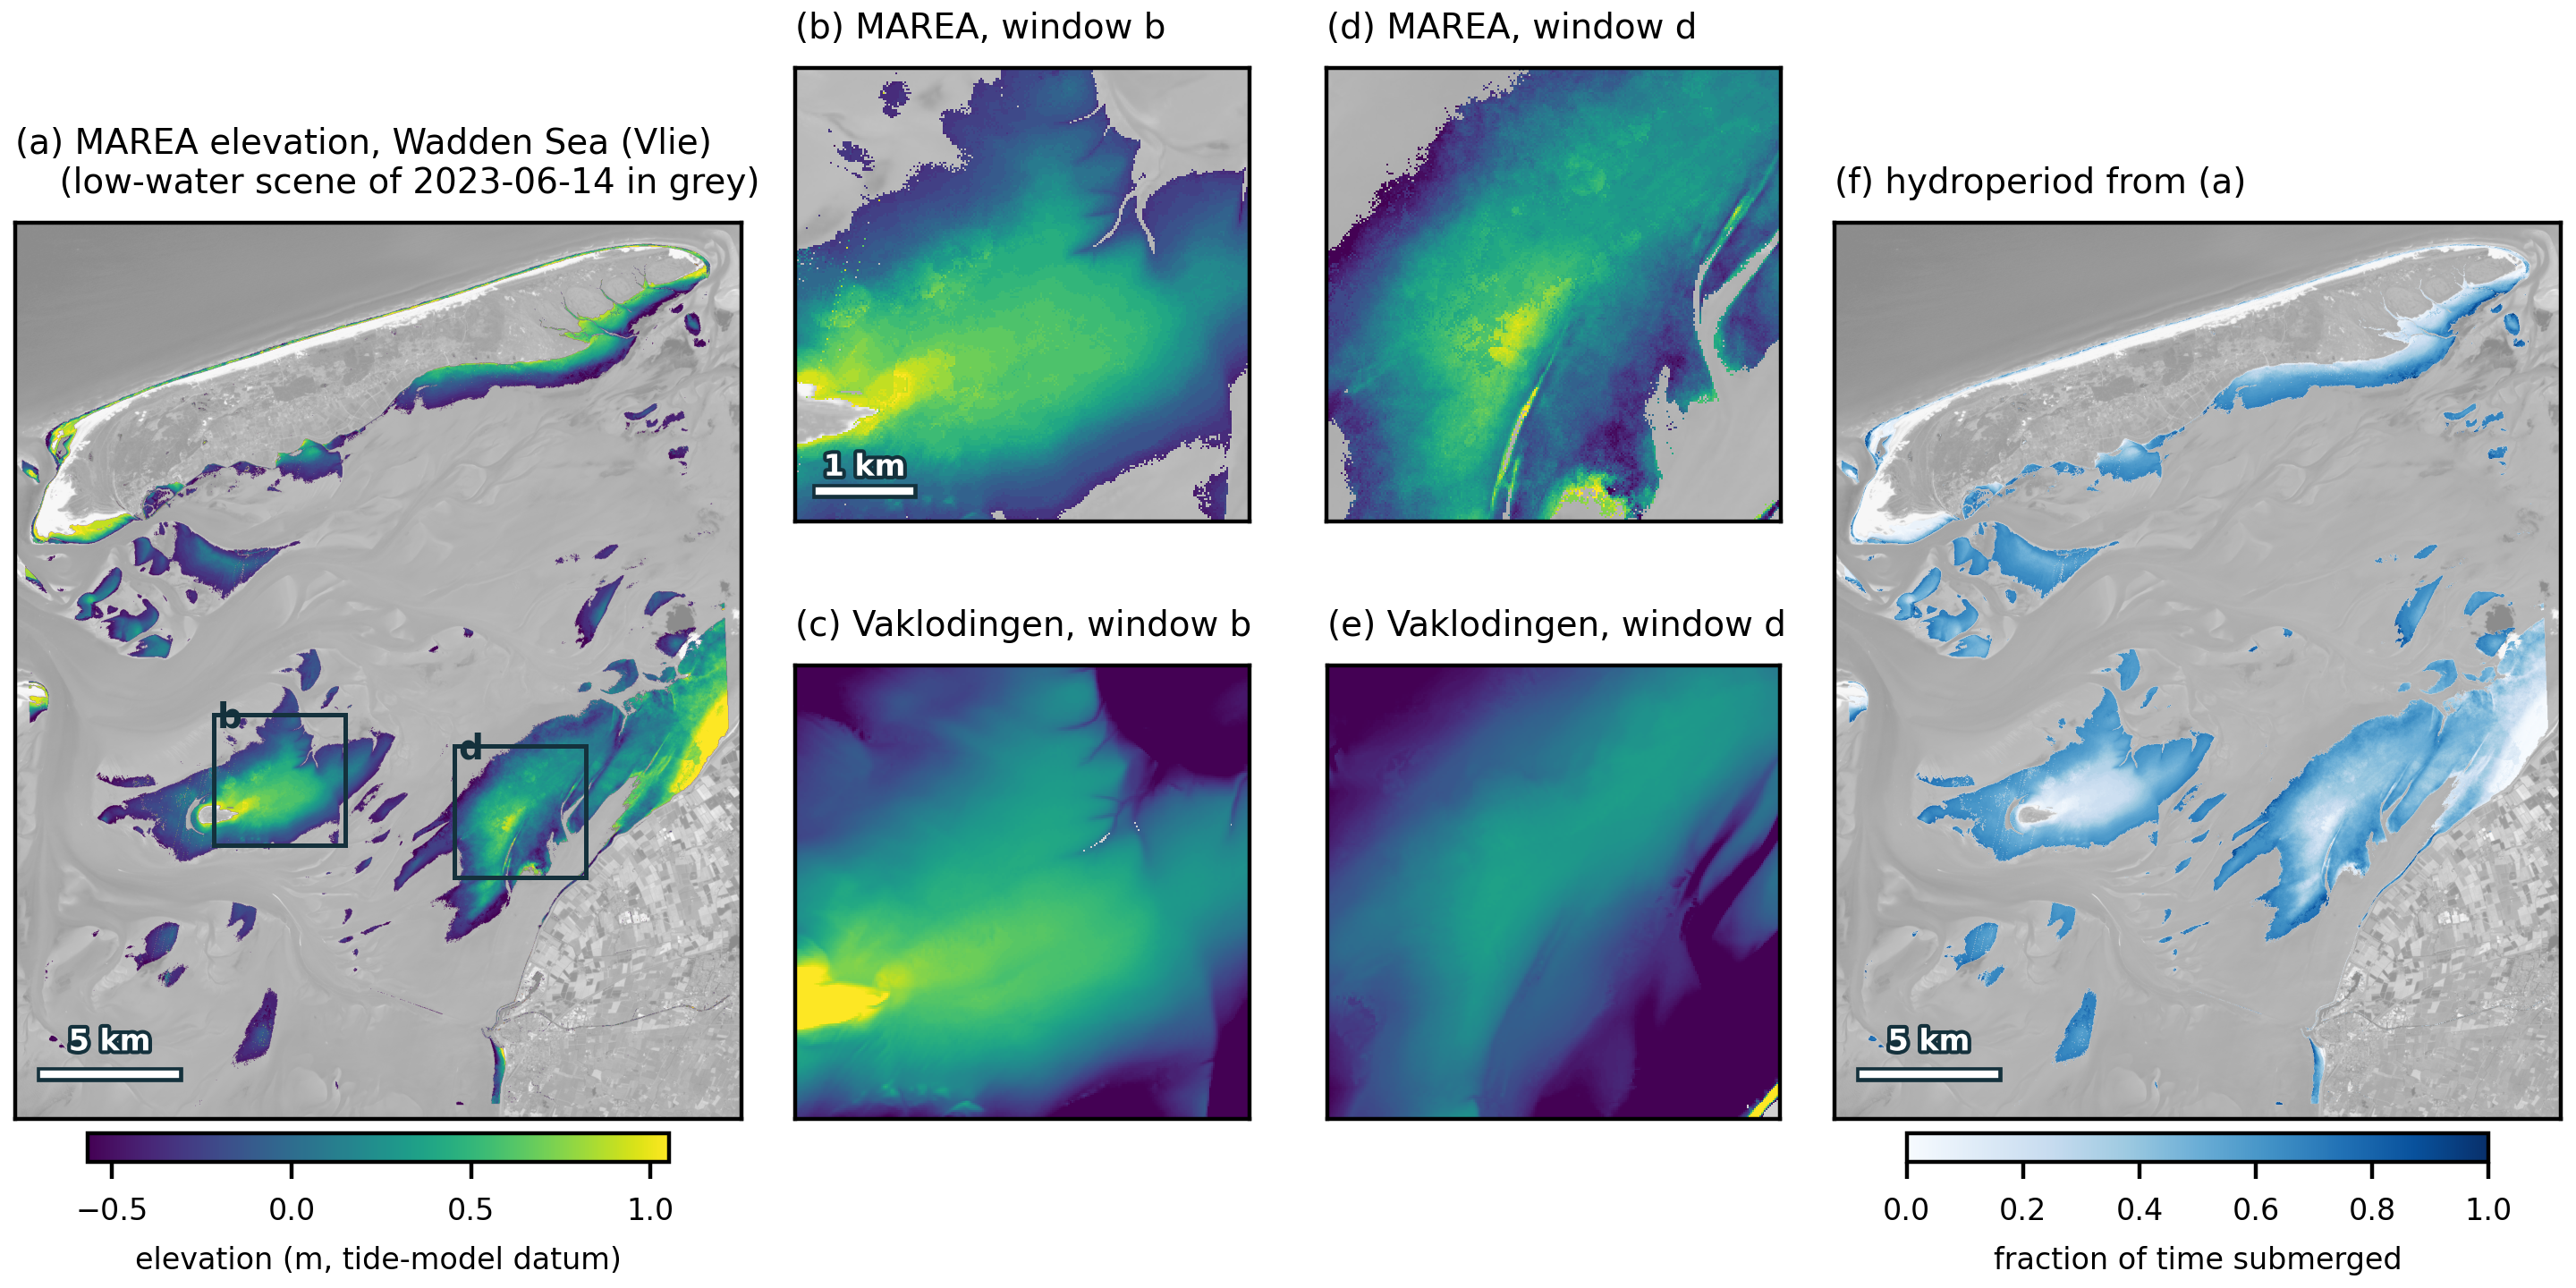
\includegraphics[width=0.94\textwidth]{fig_products.png}
\caption{The products of the Wadden Sea site (Vlie inlet to Harlingen),
2023--2025, over the clearest low-water scene of the archive in grey.
(a) The MAREA elevation map on the intertidal zone, with two zoom
windows marked; (b), (d) the windows in the MAREA map (20-m grid);
(c), (e) the same windows in the Rijkswaterstaat Vaklodingen, the
official survey of the flats and channels, one value per 20-m cell taken
cell for cell without interpolation, same colour scale, datum offset
removed; (f) the hydroperiod, the fraction of time each pixel is
submerged, from map (a) and the tide series.}
\label{fig:products}
\end{figure*}

% NUMBERS: lidar_metrics.csv (Ferrol), products_marea/lidar_external_metrics.csv
% (Villaviciosa), vaklodingen_metrics.csv / vaklodingen_by_band.csv (Dutch
% sites), run of 2026-09-23; experiments/v6_lidar_external.py assembles them.
\begin{table*}[t]
\centering
\caption{Elevation against the external references: the IGN 5~m LiDAR
DTM (PNOA) at the Spanish sites, the Rijkswaterstaat Vaklodingen at the
Dutch sites. Each map on all intertidal pixels it resolves (left) and on
those both resolve (right), Eq.~\eqref{eq:metrics}, reference inside the
tide range the maps could sample. Spanish site headers give the LiDAR
diagnostic: modal value over the intertidal mask and share of cells
within 5~cm of it, the water-surface share of the truth.}
\label{tab:external}
\footnotesize
\setlength{\tabcolsep}{4pt}
\resizebox{\textwidth}{!}{%
\begin{tabular}{@{}lrrrrrrr@{}}
\toprule
 & \multicolumn{4}{c}{all resolved pixels} & \multicolumn{3}{c}{common pixels} \\
\cmidrule(lr){2-5}\cmidrule(lr){6-8}
method & $n$ & RMSE (m) & $b$ & $r$ & RMSE (m) & $b$ & $r$ \\
\midrule
\multicolumn{8}{@{}l}{\emph{R\'ia de Villaviciosa}, IGN LiDAR --- mode $+2.00$~m, 69\,\% of cells within 5~cm, above the tide range and excluded} \\
MAREA & 7\,458 & 0.803 & 0.47 & 0.33 & 0.760 & 0.42 & -- \\
Granadeiro & 4\,477 & 0.775 & 0.32 & 0.25 & 0.767 & 0.33 & -- \\
\midrule
\multicolumn{8}{@{}l}{\emph{R\'ia de Ferrol}, IGN LiDAR --- mode $0.00$~m, 78\,\% of cells within 5~cm} \\
MAREA & 51\,716 & 0.736 & 0.46 & 0.13 & 0.648 & 0.53 & -- \\
Granadeiro & 49\,262 & 0.732 & 0.36 & 0.09 & 0.644 & 0.54 & -- \\
\midrule
\multicolumn{8}{@{}l}{\emph{Westerschelde}, Vaklodingen} \\
MAREA & 62\,181 & 0.435 & 0.76 & 0.92 & 0.385 & 0.80 & 0.94 \\
Granadeiro & 45\,005 & 0.777 & 0.78 & 0.77 & 0.776 & 0.78 & 0.78 \\
\midrule
\multicolumn{8}{@{}l}{\emph{Ems-Dollard}, Vaklodingen} \\
MAREA & 412\,565 & 0.363 & 0.65 & 0.84 & 0.327 & 0.67 & 0.86 \\
Granadeiro & 98\,953 & 0.531 & 0.39 & 0.58 & 0.521 & 0.40 & 0.58 \\
\midrule
\multicolumn{8}{@{}l}{\emph{Wadden Sea (Vlie)}, Vaklodingen} \\
MAREA & 348\,894 & 0.329 & 0.81 & 0.68 & 0.230 & 1.00 & 0.83 \\
Granadeiro & 65\,576 & 0.477 & 0.65 & 0.44 & 0.427 & 0.77 & 0.53 \\
\bottomrule
\end{tabular}}
\end{table*}

% figure fig:vaklodingen_bands is placed after the bibliography (main.tex)


% Numbers: vaklodingen_metrics.csv / vaklodingen_by_band.csv (Dutch sites),
% lidar_metrics.csv (Ferrol), run of 2026-09-23. Villaviciosa pending.
Against the Vaklodingen (Table~\ref{tab:external},
Fig.~\ref{fig:vaklodingen_bands}) MAREA is the closer map at the three
Dutch sites. In the Westerschelde it scores 0.435~m RMSE with slope 0.76
and $r = 0.92$ on 62\,000 pixels, Granadeiro 0.777~m on 45\,000. In the
Ems-Dollard MAREA scores 0.363~m with slope 0.65 and $r = 0.84$ on
413\,000 pixels; Granadeiro resolves a quarter of them at 0.531~m with
slope 0.39. In the Vlie basin MAREA scores 0.329~m with slope 0.81 on
349\,000 pixels, Granadeiro 0.477~m on 66\,000; on the pixels both
resolve, 0.230 against 0.427~m. Fig.~\ref{fig:products} shows the Vlie
map beside the Vaklodingen and the hydroperiod derived from it. The lag
carries the two large sites:
inverted without it, the same pixels score 0.565~m with slope 0.24 in
the Ems-Dollard and 0.474~m in the Vlie, and beyond 28~km of the Ems the
error falls from 0.50--0.66~m to 0.28--0.42~m with the clock.
% ^ ablation of MAREA's own clock (from the same CSVs), kept as one
% sentence; not a method row in the tables.
At the Spanish sites the LiDAR is a water surface: 78\,\% of the Ferrol
cells lie within 5~cm of 0.00~m, and inside the tide range both maps
score 0.73~m there with correlations near 0.1; in Villaviciosa 69\,\% of
the 32\,120 cells lie within 5~cm of $+2.00$~m, above the tide range
and excluded, and on the 8\,630 cells left both maps score 0.78 to
0.80~m with $r$ below 0.35. The reference discriminates nothing at
either site.

\subsection{Limitations and future work}\label{sec:limitations}

\paragraph{Gain.} A wet/dry archive fixes the phase of the interior tide,
not its amplitude (Section~\ref{sec:adoption}): gain enters only as an
external prior, and a strongly amplified tide leaves it unmeasured in the
elevations.

\paragraph{Sampling.} A sun-synchronous sensor never sees $S_2$ and
samples $M_2$ at a 14.8-day alias; the lowest spring tides never enter
the archive, so the products stop at the lowest observed level.

\paragraph{Bands and smoothing.} The lag is measured per 3-km band and
applied through a kernel of the same length, so sharper phase changes
are not resolved. Lags are applied wherever fitted, noise included, at
a cost of centimetres where no lag exists.

\paragraph{Boundary.} Lags are measured against the boundary series at
the mouth, whose phase error is absorbed into the lag while the residual
level error holds the surge and harmonics it lacks; the nearest gauge
always beat the model and their consensus.

\paragraph{Epochs and truth years.} Morphology moves, so products are
fitted per epoch of two to three years; the truths have their own dates
(the Dollard, 2020).

\paragraph{The comparison method.} Granadeiro et
al.~\cite{granadeiro2021} was reimplemented from the paper with declared
substitutions; the numbers are ours, not theirs.


\section{Conclusion}\label{sec:conclusions}
\emph{(to be written)}

\section*{Code and data availability}
\emph{(to be written from the README's data-availability table.)}

% Until the text cites them, list the whole working bibliography so the
% reference list can be checked in the PDF.
\nocite{*}
\bibliographystyle{elsarticle-num}
\bibliography{marea}

\end{document}
